\section{Strumenti utilizzati}

Per la realizzazione della tesi sono state usati i seguenti strumenti:
\paragraph{•} Arduino 
\paragraph{•} NFC Shield v2.0
\paragraph{•} NFC Tag
\paragraph{•} Java
\paragraph{•} NoSQL Database

\subsection{Arduino Uno}
Arduino è una piattaforma hardware composta da una serie di schede elettroniche dotate di un microcontrollore. È stata ideata e sviluppata nel 2003 da alcuni membri dell'Interaction Design Institute di Ivrea come strumento per la prototipazione rapida e l'utilizzo in vari ambiti, per esempio la robotica e la domotica.
\begin{center}
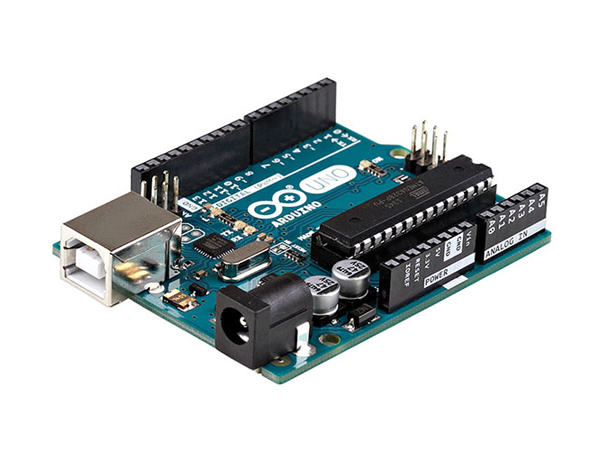
\includegraphics[scale=0.5]{arduino}
\end{center}
\subsection{NFC Shield v2.0}
Le shield sono schede che possono vengono inserite sopra l'Arduino, permettono l'estensione delle capacità della scheda stessa.La shield usata un questo progetto è quella NFC composta da un'antenna che collegandosi ad Arduino abilita la capacità di leggere/scrivere sui chip NFC
\begin{center}
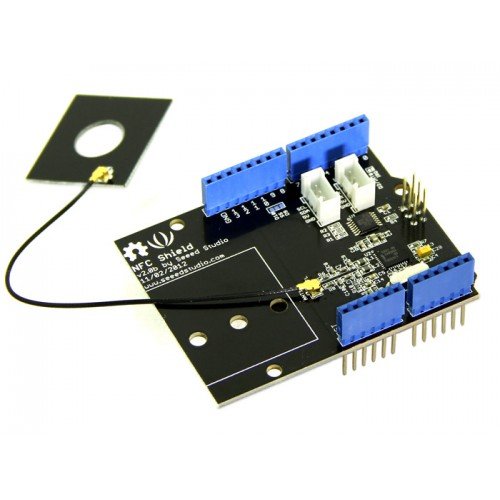
\includegraphics[scale=0.5]{shield}
\end{center}
\subsection{NFC Tag}
La tecnologia NFC  è una combinazione d'identificazione senza contatto (\textbf{RFID}) e altre tecnologie di connettività.NFC permette una comunicazione bidirezionale: quando due apparecchi NFC (initiator e target) vengono accostati entro un raggio di 4 cm, viene creata una rete peer-to-peer tra i due ed entrambi possono inviare e ricevere informazioni.
\\La tecnologia NFC opera alla frequenza di 13,56 MHz e può raggiungere una velocità di trasmissione massima di 424 kbit/s.
\\Il formato dei chip NFC usato nel progetto è \textbf{NDEF} 
\subsubsection{Tipologie di tag}
Prima di iniziare questa sezione è bene sapere che esistono solo cinque tipi di tag standardizzati e appunto per questo il loro funzionamento è garantito con gli accessori che possediamo in questo momento. I nuovi tipi di tag richiederanno una standaridzzazione e potrebbero anche richiedere un aggiornamento dell'architettura NFC che possediamo attualmente.

\paragraph{•}\textbf{Tipo 1}: il primo tipo è quello più semplice a causa di questo viene anche considerato come il più lento, ed essendo così semplice anche a livello di prezzo risulta essere molto economico. Il problema riguarda il fatto che certe funzionalità per delle applicazioni specifiche potrebbero mancare. Solitamente questi tag vengono usati per:
\subparagraph{-} Applicazioni in sola lettura
\subparagraph{-}  Accoppiamento di dispositivi bluetooth
\subparagraph{-} Lettura di un tag specifico quando c’`e ne sono tanti

\paragraph{•}\textbf{Tipo 2}:
Prima di iniziare questa sezione è bene sapere che esistono solo cinque tipi di tag standardizzati e appunto per questo il loro funzionamento è garantito con gli accessori che possediamo in questo momento. I nuovi tipi di tag richiederanno una standaridzzazione e potrebbero anche richiedere un aggiornamento dell'architettura NFC che possediamo attualmente.
\paragraph{•} \textbf{Tipo 1}: il primo tipo è quello più semplice a causa di questo viene anche considerato come il più lento, ed essendo così semplice anche a livello di prezzo risulta essere molto economico. Il problema riguarda il fatto che certe funzionalità per delle applicazioni specifiche potrebbero mancare.  Solitamente questi tag vengono usati per:
\subparagraph{-} Applicazioni in sola lettura
\subparagraph{-} Accoppiamento di dispositivi bluetooth
\subparagraph{-} Lettura di un tag specifico quando c'è ne sono tanti
\paragraph{•}\textbf{Tipo 2}: il secondo tipo è quello più popolare, perché offre ottime funzionalità per un giusto prezzo, ed inoltre riesce a raggiungere un'ampia varietà di scopi. È più veloce del tipo 1, quindi viene usato per applicazioni dove l'utente si aspetta una risposta immediata, quindi:
\subparagraph{-} Transazioni di basso valore
\subparagraph{-} Ticket per eventi
\subparagraph{-} Redirect tramite URL

\subparagraph{•}\textbf{Tipo 3}: il terzo tipo si basa su standard differenti rispetto agli altri. Vengono anche conosciuti come i tag della Sony FeliCa, sono un'innovazione giapponese e molto usata in Asia. Offre molte funzionalità però il prezzo è molto alto, vengono appunto usati molto in Giappone e per questi tipi di applicazioni:
\subparagraph{-} Biglietti
\subparagraph{-} Moneta elettronica
\subparagraph{-} Dispositivi per l'assistenza sanitaria

\paragraph{•}\textbf{Tipo 4}: il quarto tipo di tag offre la maggior memoria e flessibilità tra tutti. Il prezzo è variabile però può aggirarsi dal medio all'alto, in funzione alla quantità di memoria che vuoi. La funzione più importante di questo tag è la \textit{sicurezza}, infatti è equipaggiato con funzionalità che permettono la "true authentication". Inoltre questo tag è l'unico che supporta lo standard ISO 7816 relativo alla sicurezza, inoltre permette l'auto-modifica del contenuto NDEF. Solitamente questo tag viene usato per applicazioni di biglietteria.

\paragraph{•}\textbf{Tipo 5}: il quinto tipo offre supporto per la specifica ISO 15693, viene supportata la Modalità di Comunicazione Attiva, che permette di ottenere performance in ambito di trasferimento dei dati simili alle tecnologie RF. La distanza di lettura è uguale a quella degli altri tag NFC, solitamente questi tag vengono usati per:
\subparagraph{-} Impacchettamento di prodotti
\subparagraph{-} Biglietti
\subparagraph{-} Dispositivi per l'assistenza sanitaria

\subsubsection{Standard ISO}
Ci sono diversi standard ISO usati per la tecnologia NFC tra cui: ISO 15693, 18092 e 21481 poi ECMA 340, 352 e 356 ed ETSI TS 102 190. NFC è inoltre compatibile con la diffusa architettura delle smart card contactless, basate su ISO 14443 MIFARE e Sony FeliCa (tipo 4).

\paragraph{•} ISO 15693: Lo standard ISO 15693 utilizza la frequenza 13.56 MHz, viene offerta una distanza di lettura che può variare tra 1 metro ed 1.5 metri, poiché le carte devono operare a distanza, è richiesta la presenza di campi magnetici inferiori rispetto a quelli usati per altre carte. Inoltre a differenza di altri standard c'è una funzione di anticollisione implementata, questo serve per consentire una lettura simultanea di più card senza incorrere in errori o fail di ricezione.
\paragraph{•} ISO 18092, definisce lo standard di una smartcard contactless, viene prevalentemente usato nei sistemi RFID (pre-NFC). Questa tecnologia  viene usata con i tag di tipo 4 quindi in Giappone. Questa specifica è formata dalle ISO 15693 (vista prima) e dalla ISO 9798 che regolamenta il protocollo di comunicazione a mutuo riconoscimento, questo implica che il tag può essere letto solo da un lettore già programmato.

%\subsection{ISO 14443}
%prova \footnote{http://google.com}



%\subsection{Java}
%Java è un linguaggio di programmazione ad alto livello, orientato agli oggetti e a tipizzazione statica, specificamente progettato per essere il più possibile indipendente dalla piattaforma hardware di esecuzione (tramite compilazione in bytecode prima e interpretazione poi da parte di una JVM), la scelta di questo linguaggio è dovuta alla politica \textbf{WORA} ovvero Write Once, Run Anywhere. Infatti il risultato dell'elaborato è un file con estensione \textit{JAR} il quale rende possibile l'uso su ogni dispositivo a patto che abbia installato java
%\subsection{Eclipse}
%Eclipse è un ambiente di sviluppo integrato multi-linguaggio e multipiattaforma. Ideato da Ericsson, HP, IBM, Intel, MontaVista Software, QNX, SAP e Serena Software.
%\\Eclipse può essere utilizzato per la produzione di software di vario genere, si passa infatti da un completo IDE per il linguaggio Java (che è quello usato in questo progetto) a un ambiente di sviluppo per il linguaggio C++  e a plug-in che permettono di aggiungere molteplici funzionalità all'ambiente di sviluppo.
%\\La piattaforma di sviluppo è incentrata sull'uso di plug-in, delle componenti software ideate per uno specifico scopo, per esempio la generazione di diagrammi UML, ed in effetti tutta la piattaforma è un insieme di plug-in, versione base compresa, e chiunque può sviluppare e modificare i vari plug-in. Nella versione base è possibile programmare in Java, usufruendo di comode funzioni di aiuto quali: completamento automatico, suggerimento dei tipi di parametri dei metodi, possibilità di accesso diretto a CVS e riscrittura automatica del codice (Refactoring).
%\\Essendo scritto in Java, Eclipse è disponibile per le piattaforme Linux, macOS, Windows e altri sistemi operativi.